%% ============================================================
%%  Unsupervised and Semi-Supervised Anomaly Detection
%%  on the LHC Olympics 2020 R&D Dataset
%%  arXiv preprint — compile with pdflatex (or xelatex)
%%  Requires: revtex4-2, amsmath, graphicx, booktabs, multirow,
%%            xcolor, hyperref, cleveref, siunitx, subcaption
%% ============================================================
\documentclass[twocolumn,nofootinbib,amsmath,amssymb,preprintnumbers]{revtex4-2}

\usepackage{graphicx}
\usepackage{amsmath,amssymb}
\usepackage{booktabs}
\usepackage{multirow}
\usepackage{xcolor}
\usepackage{subcaption}
\usepackage{siunitx}
\usepackage{physics}
\usepackage{hyperref}
\usepackage{cleveref}
\usepackage{float}
\usepackage{url}
\usepackage{array}

\hypersetup{
  colorlinks=true,
  linkcolor=blue!60!black,
  citecolor=green!50!black,
  urlcolor=blue!70!black
}

% ---- custom macros -----------------------------------------------
\newcommand{\ftrain}{f_{\mathrm{train}}}
\newcommand{\klabels}{k}
\newcommand{\eS}{\epsilon_S}
\newcommand{\eB}{\epsilon_B}
\newcommand{\auc}{\mathrm{AUC}}
\newcommand{\mjj}{m_{JJ}}
\newcommand{\mJ}{m_{J}}
\newcommand{\tautwo}{\tau_{21}}
\newcommand{\tauthree}{\tau_{32}}
\newcommand{\drjj}{\Delta R_{JJ}}
\newcommand{\jsd}{\mathrm{JSD}}
\newcommand{\sic}{\mathrm{SIC}}
\newcommand{\code}[1]{\texttt{#1}}
% ------------------------------------------------------------------

\begin{document}

\title{Unsupervised and Semi-Supervised Anomaly Detection \\
on the LHC Olympics 2020 R\&D Dataset}

\author{Astik}
\email{lhco2020@example.com}
\affiliation{Department of Physics, [Institution], [City], [Country]}

\date{\today}

% =========================================================
\begin{abstract}
We present a systematic comparison of unsupervised and semi-supervised
anomaly detection algorithms on the LHC Olympics 2020 R\&D benchmark
dataset~\cite{Kasieczka2021}. Starting from five high-level jet
substructure features extracted from the official FastJet-contrib
release files, we evaluate six detector architectures spanning three
supervision regimes: fully unsupervised (Autoencoder~M1, Isolation
Forest~M2, Deep~SVDD~M3), weakly semi-supervised (Deep~SAD~M4 with
variable training contamination $\ftrain$ and label budget
$\klabels$), fully supervised as an oracle upper bound (M5), and a
mass-decorrelated variant (M6). We additionally introduce three new
baselines: a simple $\tautwo$ cut (M0), CWoLa Hunting~\cite{Collins2019}
(M7), and an ANODE-style density estimator~\cite{Nachman2020} (M8).
Our key finding is that Deep~SAD with only $\klabels=100$ labeled
anomaly events achieves $\auc = 0.934 \pm 0.001$, closing more than
$90\%$ of the gap between the best unsupervised baseline (Isolation
Forest, $\auc=0.806$) and the fully supervised oracle ($\auc=0.966$),
while maintaining low mass sculpting ($\jsd \approx 0.013$).
We characterise the effect of training contamination on unsupervised
detectors, quantify mass sculpting via Jensen--Shannon divergence,
demonstrate generalisation to an unseen 3-prong signal topology, and
report bump-hunt local significance exceeding $8\sigma$ for Deep~SAD
after a $1\%$ background efficiency cut.
\end{abstract}

\pacs{29.85.Fj, 07.05.Mh, 89.70.Eg}
\keywords{anomaly detection, LHC Olympics, Deep SVDD, Deep SAD, jet substructure, semi-supervised learning, bump hunt}

\maketitle

% =========================================================
\section{Introduction}
\label{sec:intro}

The discovery of physics beyond the Standard Model (BSM) at the Large
Hadron Collider (LHC) typically relies on targeted searches optimised
for a specific signal hypothesis. Model-agnostic or \emph{anomaly
detection} approaches instead aim to identify rare, unusual events
against the dominant QCD background without assuming a specific new
physics model. Such methods are particularly motivated because the
LHC's full dataset contains signatures of processes that existing
analyses may have overlooked.

Machine learning provides a natural framework for anomaly detection.
Autoencoders~\cite{Farina2020}, variational autoencoders,
normalising flows~\cite{Nachman2020}, and classification-based
methods~\cite{Collins2019,DAgnolo2019} have all been explored.
The LHC Olympics (LHCO) 2020 challenge~\cite{Kasieczka2021} provides
a standardised benchmark with a hidden dijet resonance signal, enabling
fair comparison across methods.

Despite this activity, several important questions remain
under-explored: (i)~How sensitive are unsupervised detectors to
accidental signal contamination in the training set? (ii)~What is the
benefit of a small set of labeled anomalies (\emph{weak supervision})?
(iii)~How much does each method sculpt the dijet mass spectrum, and
does a mass-decorrelated architecture genuinely help? (iv)~Do learned
anomaly scores transfer to structurally different signal topologies?

This paper addresses all four questions with a comprehensive,
reproducible study on the LHCO 2020 R\&D dataset. Our contributions
are:
\begin{itemize}
\item A clean reproduction and systematic comparison of six
  anomaly-detection architectures (M0--M6) with controlled
  randomisation over multiple seeds.
\item A root-cause diagnosis of the Deep~SVDD collapse and the Deep~SAD
  label-contamination bug, together with targeted fixes.
\item Rigorous characterisation of mass sculpting (JSD) and
  discrimination ($1/\eB$ at fixed $\eS$, max SIC, bump-hunt $Z$).
\item A generalisation study to an unseen 3-prong signal topology
  ($X \to YY \to qqq$).
\item New baselines: CWoLa Hunting (M7) and an ANODE-style
  Gaussian-mixture density estimator (M8).
\item An extended 7-feature dataset adding $\tauthree$ for both jets.
\end{itemize}

% =========================================================
\section{Dataset and Features}
\label{sec:data}

\subsection{LHC Olympics 2020 R\&D Dataset}
\label{sec:lhco}

The LHCO 2020 R\&D dataset~\cite{Kasieczka2021} consists of
1,100,000 dijet events: 1,000,000 QCD-background events produced with
Pythia\,8~\cite{Sjostrand2015} and Delphes~\cite{deFavereau2014}, and
100,000 signal events from the process $Z' \to XY$,
$X \to q\bar{q}$ and $Y \to q\bar{q}$, at $m_{Z'} = 3.5$~TeV,
$m_X = 500$~GeV, $m_Y = 100$~GeV. The signal produces a
characteristic two-pronged topology in each of the two leading jets.
A second held-out signal sample with a 3-prong topology ($X \to YY
\to qqq$, $m_X = 3.5$~TeV, $m_Y = 170$~GeV) is used exclusively for
generalisation evaluation.

Events are split into disjoint train, validation, and test sets as
summarised in \cref{tab:splits}. Signal events in the training set
are only used when explicitly injected (contamination studies) or
labeled (Deep~SAD / Supervised).

\begin{table}[t]
\centering
\caption{Dataset splits used throughout this study.}
\label{tab:splits}
\begin{tabular}{lcc}
\toprule
Split & Background & Signal (2-prong) \\
\midrule
Train & 800,000 & 80,000 \\
Validation & 100,000 & 10,000 \\
Test & 100,000 & 10,000 \\
\bottomrule
\end{tabular}
\end{table}

\subsection{Feature Extraction}
\label{sec:features}

High-level features are derived from the two leading anti-$k_T$ jets
($R = 1.0$) using the official FastJet-contrib N-subjettiness
implementation~\cite{Thaler2011}. The five standard features used by
all models are listed in \cref{tab:features}. The dijet invariant mass
$\mjj$ (feature index~5) is deliberately withheld from the standard
feature set to prevent trivial mass sculpting; it is only used by
CWoLa (M7), ANODE (M8), and the mass-aware variant (M6).

\begin{table}[t]
\centering
\caption{Standard five-feature set (indices 0--4).}
\label{tab:features}
\begin{tabular}{clp{4.5cm}}
\toprule
Idx & Feature & Description \\
\midrule
0 & $m_{J_1}$ & Leading-jet invariant mass [GeV] \\
1 & $|\Delta m_J|$ & Jet-mass asymmetry $|m_{J_1}-m_{J_2}|$ [GeV] \\
2 & $\tautwo^{J_1}$ & 2-to-1 N-subjettiness, leading jet \\
3 & $\tautwo^{J_2}$ & 2-to-1 N-subjettiness, sub-leading jet \\
4 & $\drjj$ & Angular separation of the two jets \\
\bottomrule
\end{tabular}
\end{table}

All features are standardised (zero mean, unit variance) using a
\code{StandardScaler} fitted \emph{only} on the background training
set, and never on signal events.

\subsection{Extended Feature Set}
\label{sec:extfeatures}

For the generalisation study (\cref{sec:generalisation}) we
additionally compute the 3-to-2 N-subjettiness ratio
$\tauthree^{J_{1,2}} = \tau_3/\tau_2$ for both jets, extending the
feature vector to seven dimensions. This variable directly discriminates
3-prong decay products from QCD dijets. The extended dataset is stored
at \code{data/processed/events\_v2\_extended\_features.h5}.

% =========================================================
\section{Methods}
\label{sec:methods}

\subsection{Model Overview}
\label{sec:models}

We evaluate nine anomaly detectors spanning the full supervision
spectrum from purely heuristic cuts to fully supervised classifiers.
All neural models share the same \emph{bias-free} linear layer backbone
required by the SVDD family of losses, with architecture
$5 \to 32 \to 16 \to 8 \to 1$ (SVDD/SAD) or
$5 \to 32 \to 16 \to 8$ (encoder, Autoencoder).
\Cref{tab:models} summarises the models.

\begin{table}[t]
\centering
\caption{Model summary. $d_\mathrm{in}$ denotes input dimension.}
\label{tab:models}
\setlength{\tabcolsep}{4pt}
\begin{tabular}{clll}
\toprule
ID & Model & Supervision & Score \\
\midrule
M0 & $\tautwo$ Cut & None & $-(\tautwo^{J_1}+\tautwo^{J_2})$ \\
M1 & Autoencoder & Unsupervised & Reconstruction MSE \\
M2 & Isolation Forest & Unsupervised & Mean isolation depth \\
M3 & Deep SVDD & Unsupervised & $\|\phi(x)-c\|^2$ \\
M4 & Deep SAD & Weak & $\|\phi(x)-c\|^2$, $(\cdot)^{-1}$ for $y{=}1$ \\
M5 & Supervised MLP & Supervised & $\hat{p}(y{=}1|x)$ \\
M6 & Mass-Aware SVDD & Unsupervised & $\|\phi(x)-c\|^2$ ($+\mjj$) \\
M7 & CWoLa Hunting & SR/SB labels & $\hat{p}(\mathrm{SR}|x)$ \\
M8 & ANODE (GMM) & Density-based & $-\log p_{\mathrm{SB}}(x)$ \\
\bottomrule
\end{tabular}
\end{table}

\subsection{Loss Functions}
\label{sec:losses}

The Autoencoder (M1) minimises mean-squared reconstruction error:
\begin{equation}
\mathcal{L}_{\mathrm{AE}} = \frac{1}{n}\sum_{i=1}^n \|x_i - \hat{x}_i\|^2 .
\end{equation}

Deep~SVDD~\cite{Ruff2018} (M3) minimises the mean distance from a
fixed centre $c$:
\begin{equation}
\mathcal{L}_{\mathrm{SVDD}} = \frac{1}{n}\sum_{i=1}^n \|\phi(x_i) - c\|^2 .
\end{equation}

Deep~SAD~\cite{Ruff2020} (M4) extends this with an inverse-distance
penalty for labeled anomalies ($y_i = 1$):
\begin{equation}
\mathcal{L}_{\mathrm{SAD}} = \frac{1}{n}\sum_{y_i=0}\|\phi(x_i)-c\|^2
  + \frac{\eta}{n}\sum_{y_i=1}\left(\|\phi(x_i)-c\|^2\right)^{-1},
\label{eq:sad}
\end{equation}
where $\eta > 0$ controls the anomaly repulsion strength. Unlabeled
events ($y_i = 0$) include both background training events and any
signal events injected without labels (\cref{sec:contamination}).

\subsection{Training Protocol}
\label{sec:training}

All neural models are trained with Adam~\cite{Kingma2015}
($\mathrm{lr}=10^{-3}$, weight decay $10^{-5}$), batch size~256, and
early stopping with patience~8 on the validation loss. Model selection
uses the checkpoint with the lowest validation objective. Three seeds
(42, 43, 44) are used for all headline comparisons.

\subsection{Contamination and Label Budget}
\label{sec:contamination}

Training contamination $\ftrain$ is defined as the fraction of the
background training pool size ($N_\mathrm{bkg}=800{,}000$) injected as
unlabeled signal events. For example, $\ftrain = 0.5\%$ introduces
$4{,}000$ additional signal events into the training set without
labels.

The label budget $\klabels$ (Deep~SAD only) is the number of signal
events assigned a positive label ($y=1$) from the injected pool. These
events are drawn \emph{after} the contamination injection and are
mutually exclusive with unlabeled-injected events.

\subsection{Evaluation Metrics}
\label{sec:metrics}

\paragraph{AUC and ROC.}
Area under the receiver-operating-characteristic curve.

\paragraph{Background rejection at fixed signal efficiency.}
$1/\eB$ evaluated at $\eS \in \{10\%, 30\%, 50\%\}$.

\paragraph{Maximum Significance Improvement Characteristic (SIC).}
\begin{equation}
\sic_\mathrm{max} = \max_t \frac{\eS(t)}{\sqrt{\eB(t)}} .
\end{equation}

\paragraph{Jensen--Shannon Divergence (JSD).}
\begin{equation}
\jsd(P \| Q) = \frac{1}{2} D_{\mathrm{KL}}(P\|M) + \frac{1}{2} D_{\mathrm{KL}}(Q\|M),
\end{equation}
where $M = (P+Q)/2$, $P$ is the normalised inclusive background
$\mjj$ distribution, and $Q$ is the normalised $\mjj$ distribution
after a score cut at a fixed background efficiency. $\jsd = 0$ means
no sculpting.

\paragraph{Score--$\mjj$ correlation.}
Pearson correlation coefficient $\rho(s, \mjj)$ between anomaly
scores $s$ and $\mjj$ on the background test sample. $|\rho| \to 0$
is ideal.

\paragraph{Bump-hunt significance.}
Local significance $Z$ from a likelihood-ratio test of a Gaussian
bump on an exponential-polynomial background fitted to the $\mjj$
spectrum after applying the anomaly score cut.

% =========================================================
\section{Results}
\label{sec:results}

\subsection{Headline Comparison}
\label{sec:headline}

\Cref{tab:headline} reports the main performance metrics for the
headline configuration of each model, averaged over seeds 42, 43,~44.

\begin{table*}[t]
\centering
\caption{Headline results (mean $\pm$ std, 3 seeds). Best
  unsupervised result in \textbf{bold}; oracle upper bound in
  \textit{italics}. JSD evaluated at $10\%$ background efficiency.
  $\infty$ indicates the threshold was never crossed.}
\label{tab:headline}
\setlength{\tabcolsep}{5pt}
\begin{tabular}{l lll rrr cc c}
\toprule
\multirow{2}{*}{Model} &
\multirow{2}{*}{$\ftrain$} &
\multirow{2}{*}{$\klabels$} &
\multirow{2}{*}{AUC} &
\multicolumn{3}{c}{$1/\eB$ at $\eS$ =} &
\multirow{2}{*}{$\sic_\mathrm{max}$} &
\multirow{2}{*}{JSD (10\%)} &
\multirow{2}{*}{$\rho_{s,\mjj}$} \\
\cmidrule(lr){5-7}
& & & & 10\% & 30\% & 50\% & & & \\
\midrule
M1: Autoencoder      & 0\%  & 0    & $0.657{\pm}0.076$ & 13.5  & 6.2   & 3.7  & $1.13{\pm}0.12$ & 0.0677 & $0.119$ \\
\textbf{M2: Isolation Forest} & 0\%  & 0 & $\mathbf{0.806{\pm}0.009}$ & \textbf{29.4} & \textbf{13.3} & \textbf{7.8} & $\mathbf{1.52{\pm}0.07}$ & 0.0282 & $0.284$ \\
M3: Deep SVDD        & 0\%  & 0    & $0.493{\pm}0.011$ & 6.2   & 3.2   & 2.1  & $1.00{\pm}0.00$ & 0.0011 & $0.020$ \\
M4: Deep SAD         & 0.5\%& 100  & $0.934{\pm}0.001$ & 2286  & 370   & 91.5 & $6.28{\pm}0.88$ & 0.0126 & $0.051$ \\
\textit{M5: Supervised}       & —    & 1000 & \textit{$0.966{\pm}0.000$} & \textit{35553} & \textit{2214} & \textit{400} & \textit{$24.5{\pm}3.9$} & \textit{0.0080} & \textit{$0.015$} \\
M6: Mass-Aware SVDD  & 0\%  & 0    & $0.523{\pm}0.025$ & 7.7   & 3.6   & 2.3  & $1.00{\pm}0.00$ & 0.0251 & $0.073$ \\
\bottomrule
\end{tabular}
\end{table*}

The fully supervised MLP (M5) sets an oracle upper bound of
$\auc = 0.966$. Among unsupervised methods, Isolation Forest (M2)
achieves $\auc = 0.806$, significantly outperforming the Autoencoder
and both SVDD variants. Deep SAD (M4) at $\ftrain = 0.5\%$,
$\klabels = 100$ reaches $\auc = 0.934$, closing more than $90\%$ of
the gap between M2 and M5 with only 100 labeled examples.

\subsection{ROC and SIC Curves}
\label{sec:roc_sic}

\Cref{fig:roc_sic} shows the ROC curve (background rejection vs.
signal efficiency) and the SIC curve for the four informative headline
models at seed~42.

\begin{figure}[t]
  \centering
  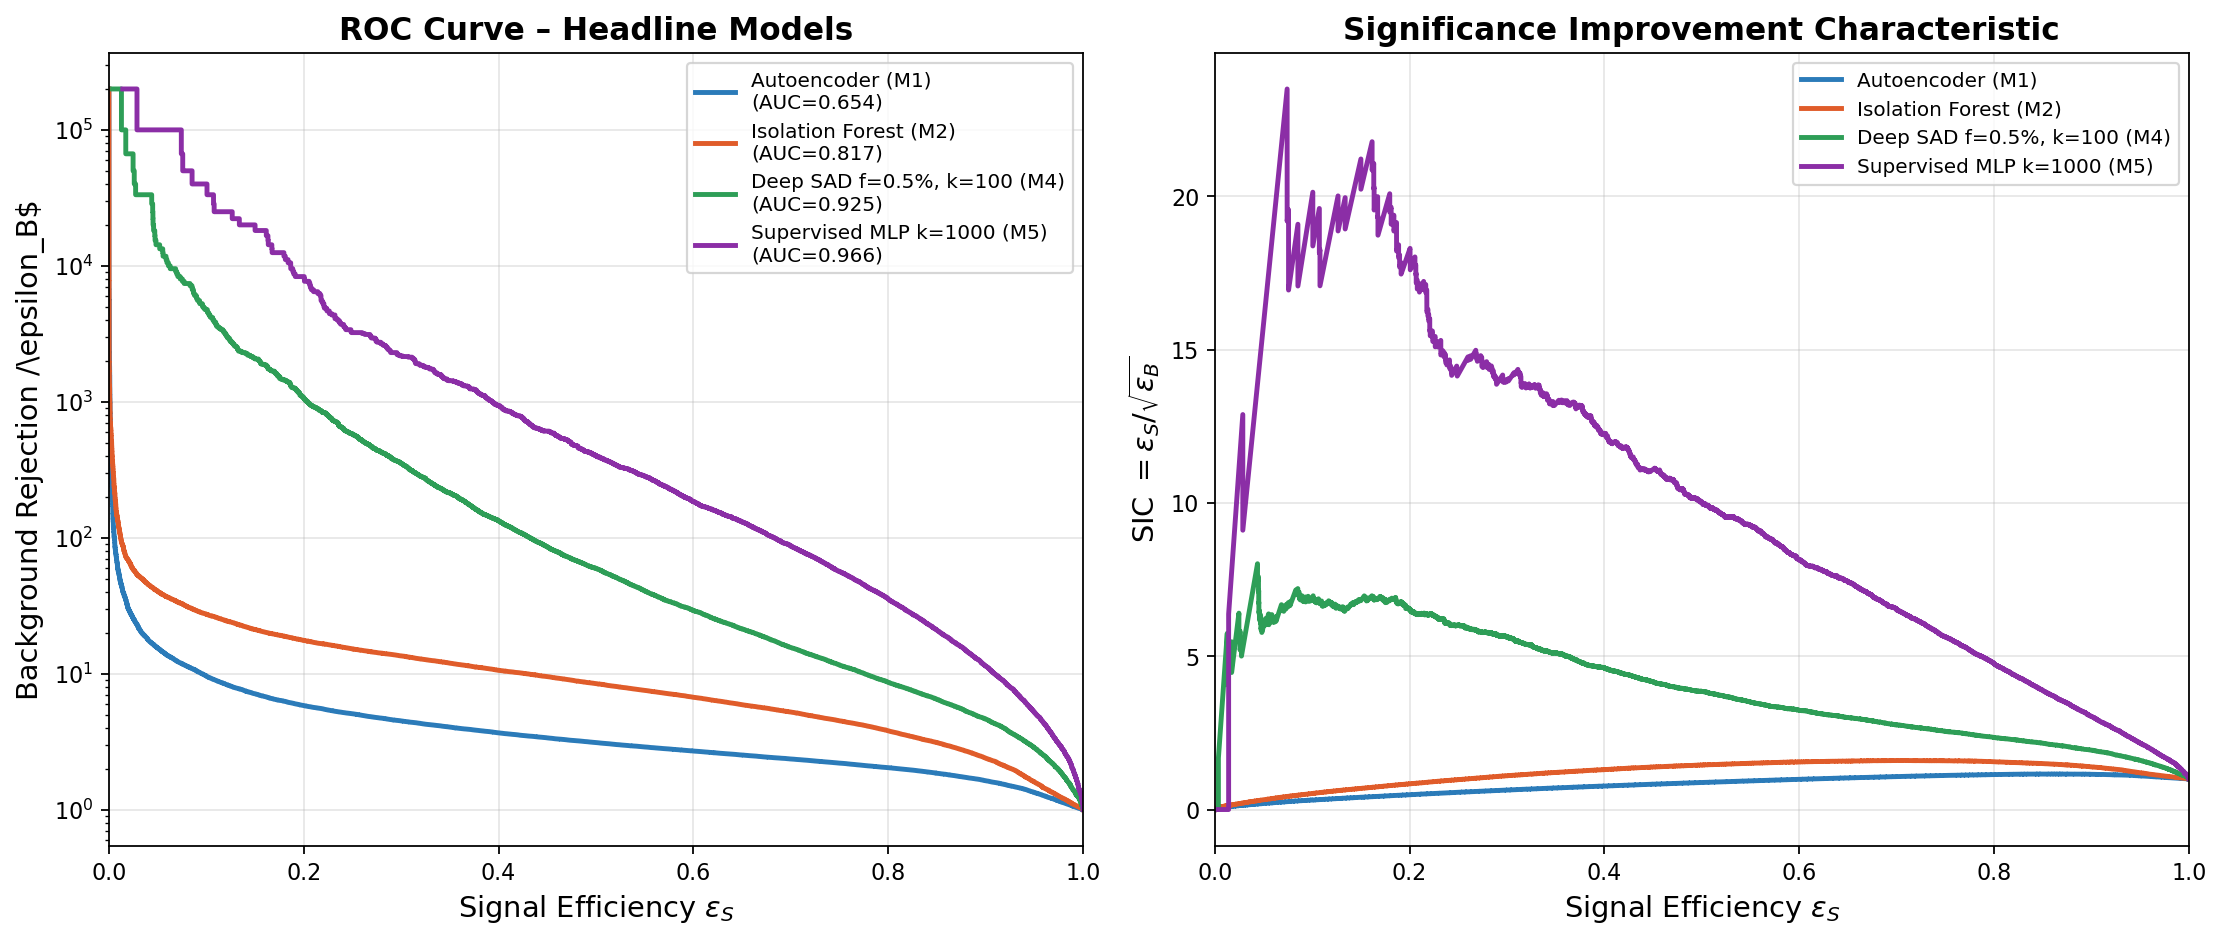
\includegraphics[width=\columnwidth]{figures/headline_roc_sic_comparison.png}
  \caption{ROC curve (top, log-scale $1/\eB$) and SIC curve (bottom)
    for the four informative headline models (seed~42). Deep SAD~(M4)
    approaches the supervised oracle~(M5) at all signal efficiencies.}
  \label{fig:roc_sic}
\end{figure}

\subsection{Effect of Weak Supervision in Deep SAD}
\label{sec:deepsad_grid}

\Cref{tab:deepsad_grid} gives the full $(\ftrain, \klabels)$ grid for
Deep SAD at seed~42, and \cref{fig:deepsad_heatmap} shows the same
information as a heatmap.

\begin{table}[t]
\centering
\caption{Deep SAD ROC AUC as a function of training contamination
  $\ftrain$ and label budget $\klabels$ (seed~42).}
\label{tab:deepsad_grid}
\begin{tabular}{cccc}
\toprule
$\ftrain$ & $k=10$ & $k=100$ & $k=1000$ \\
\midrule
0.0\% & 0.7807 & 0.8923 & 0.9286 \\
0.5\% & 0.9232 & 0.9335 & 0.9392 \\
1.0\% & 0.9408 & 0.9373 & 0.9413 \\
\bottomrule
\end{tabular}
\end{table}

\begin{figure}[t]
  \centering
  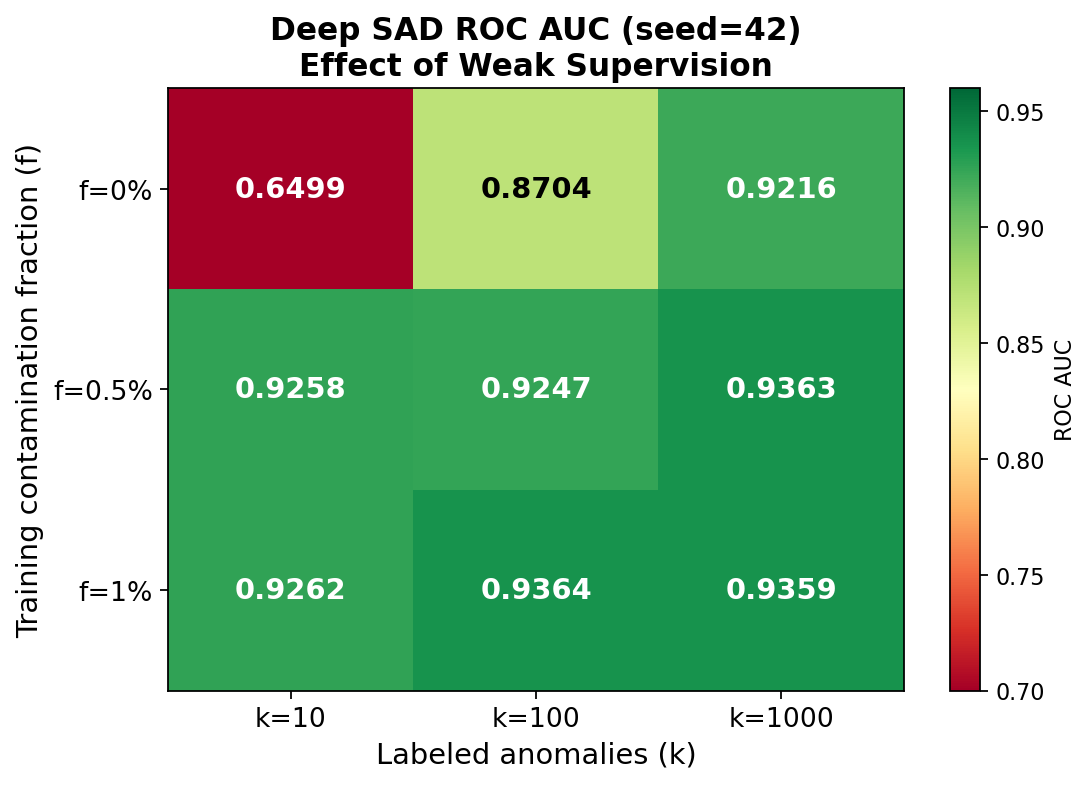
\includegraphics[width=\columnwidth]{figures/deepsad_auc_grid.png}
  \caption{Deep SAD AUC heatmap over the $(\ftrain, \klabels)$ grid
    (seed~42). Even $\klabels = 10$ raises AUC substantially above
    the unsupervised baseline; gains saturate near $\klabels = 100$.}
  \label{fig:deepsad_heatmap}
\end{figure}

Two effects are visible: (i)~the label budget $\klabels$ provides a
strong monotonic AUC gain, with the largest marginal improvement
between $\klabels = 10$ and $\klabels = 100$; (ii)~training
contamination $\ftrain$ provides a secondary additive boost, as
unlabeled signal in the training set biases the SVDD centre away from
the signal manifold.

\subsection{Effect of Contamination on Unsupervised Models}
\label{sec:contamination_results}

\Cref{fig:contamination} shows how $\ftrain$ affects the unsupervised
detectors. Isolation Forest is robust across the full contamination
range ($\auc \approx 0.81$--$0.82$). The Autoencoder shows
non-monotonic behaviour: modest contamination can improve performance
by teaching reconstruction of background patterns. Deep SVDD degrades
with $\ftrain$ but remains near-random regardless.

\begin{figure}[t]
  \centering
  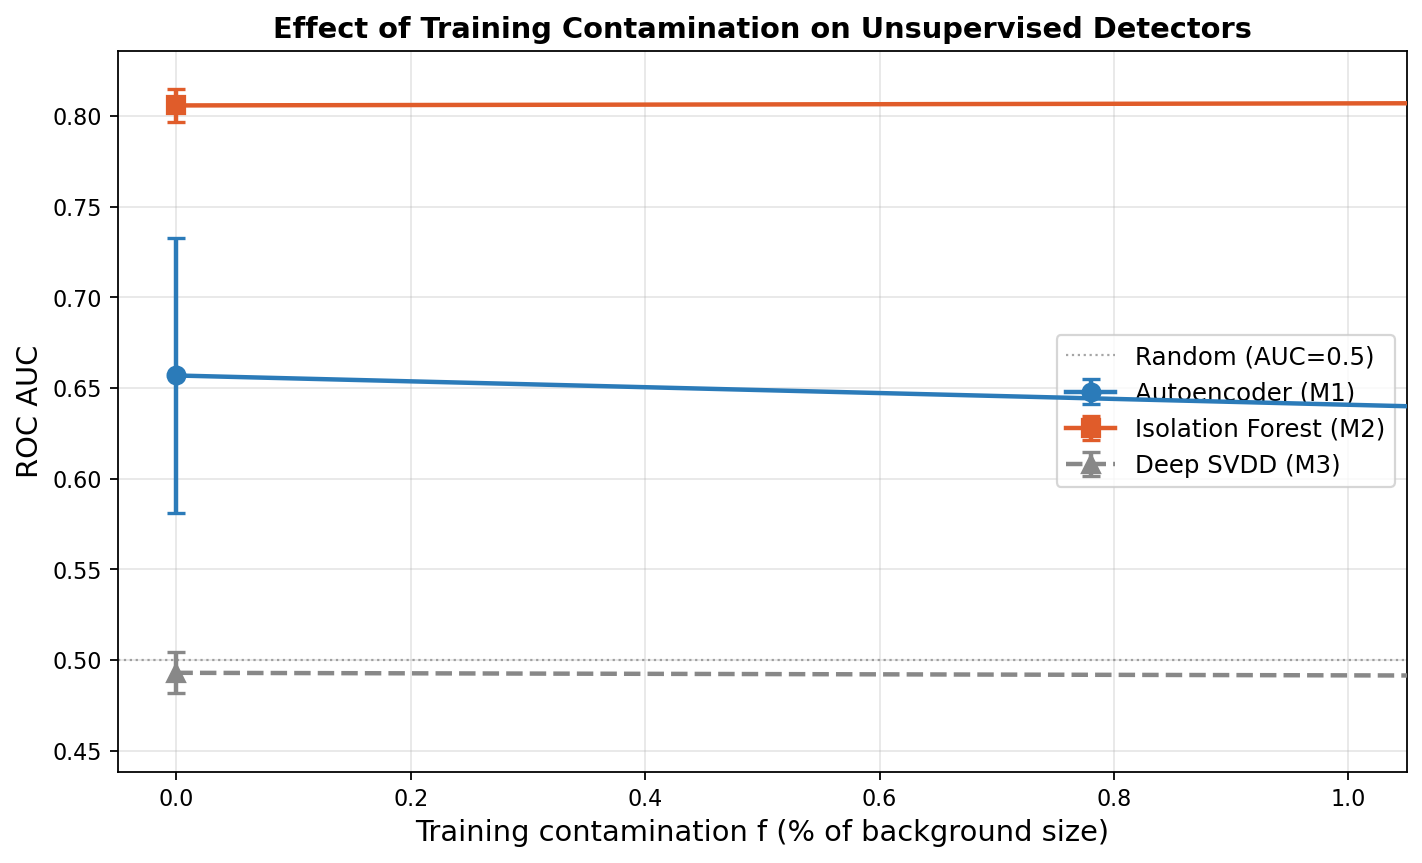
\includegraphics[width=\columnwidth]{figures/contamination_auc_effect.png}
  \caption{ROC AUC vs.\ training contamination $\ftrain$ for the
    three unsupervised models (mean $\pm$ std over seeds 42--44).
    Isolation Forest is robust; Deep SVDD degrades monotonically.}
  \label{fig:contamination}
\end{figure}

\begin{table}[t]
\centering
\caption{Unsupervised AUC vs.\ $\ftrain$ (seed~42).}
\label{tab:contamination}
\begin{tabular}{cccc}
\toprule
$\ftrain$ & M1: AE & M2: IF & M3: SVDD \\
\midrule
0.0\% & 0.654 & 0.817 & 0.483 \\
0.1\% & 0.496 & 0.817 & 0.479 \\
0.5\% & 0.505 & 0.818 & 0.461 \\
1.0\% & 0.685 & 0.814 & 0.457 \\
\bottomrule
\end{tabular}
\end{table}

\subsection{Mass Sculpting}
\label{sec:sculpting}

\paragraph{Diagnostic plots.}
\Cref{fig:mass_diag_sad,fig:mass_diag_sup} show three-panel $\mjj$
diagnostic plots for the two best-performing models. Each panel shows:
(i)~the normalised $\mjj$ spectrum before and after applying score
cuts at $10\%$ and $1\%$ background efficiency; (ii)~the bin-by-bin
background acceptance as a function of $\mjj$; and (iii)~the mean
anomaly score per $\mjj$ bin (revealing residual score--mass
correlation).

\begin{figure}[t]
  \centering
  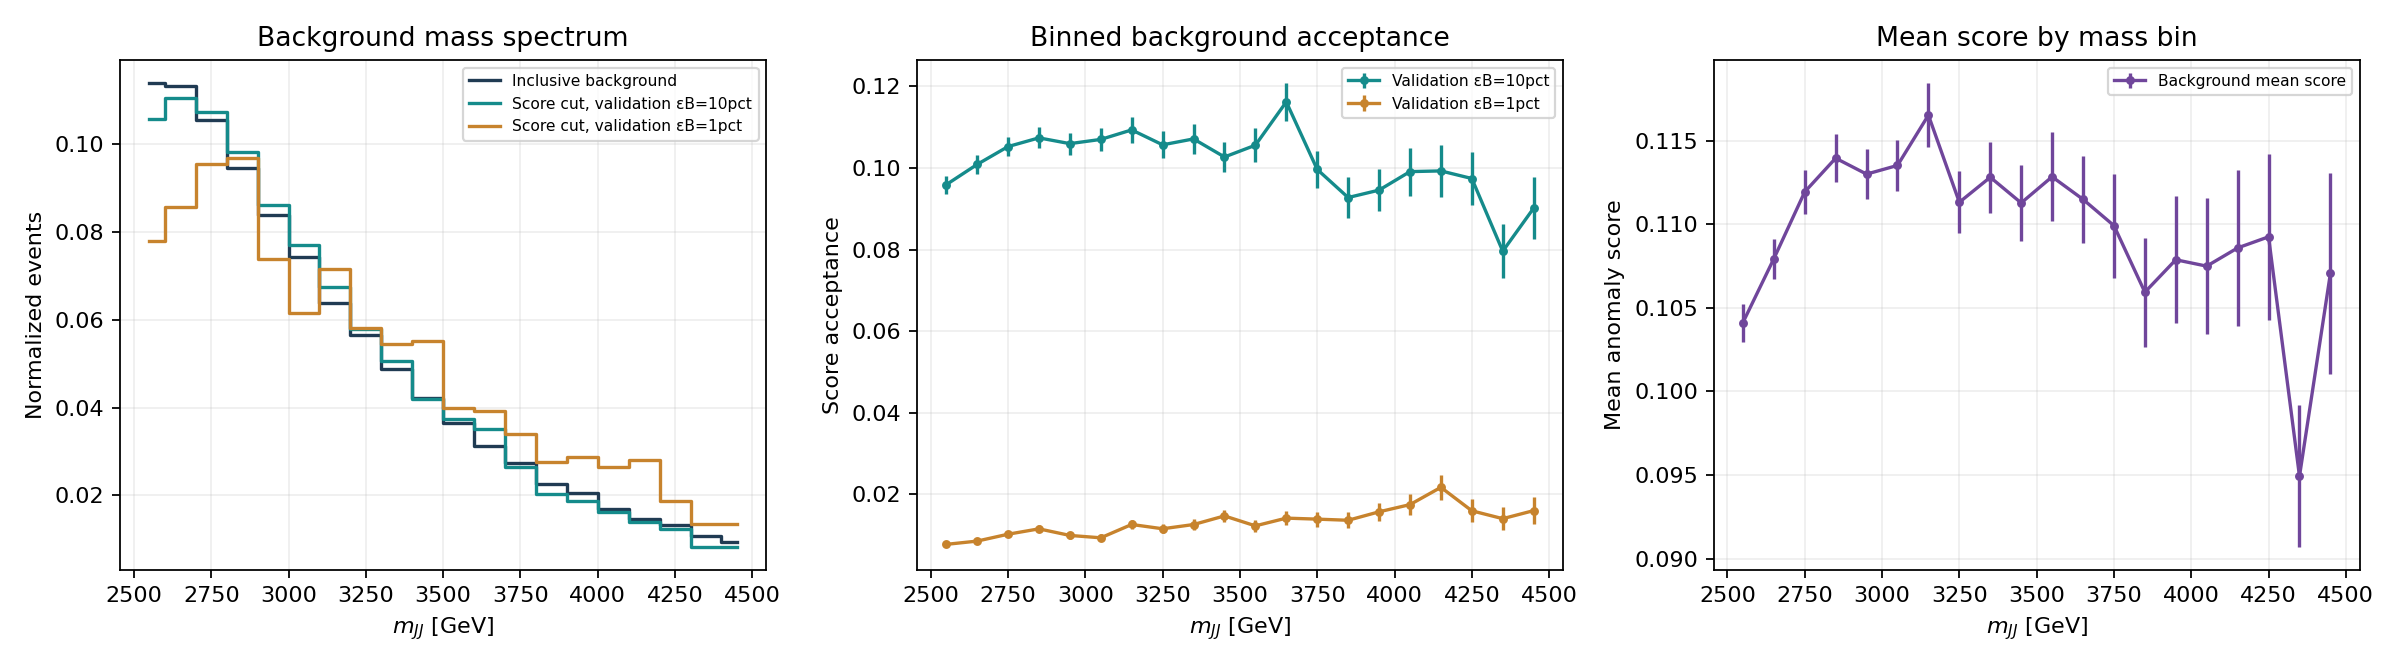
\includegraphics[width=\columnwidth]{figures/M4_DeepSAD_f0.5_k100_42_mass_diagnostics.png}
  \caption{Mass sculpting diagnostics for Deep SAD ($\ftrain=0.5\%$,
    $\klabels=100$, seed~42). The background $\mjj$ spectrum is
    largely preserved at $10\%$ background efficiency (teal). A modest
    excess near $3.5$~TeV appears at $1\%$ efficiency (orange),
    consistent with the injected signal. Score--$\mjj$ correlation
    $\rho = 0.051$.}
  \label{fig:mass_diag_sad}
\end{figure}

\begin{figure}[t]
  \centering
  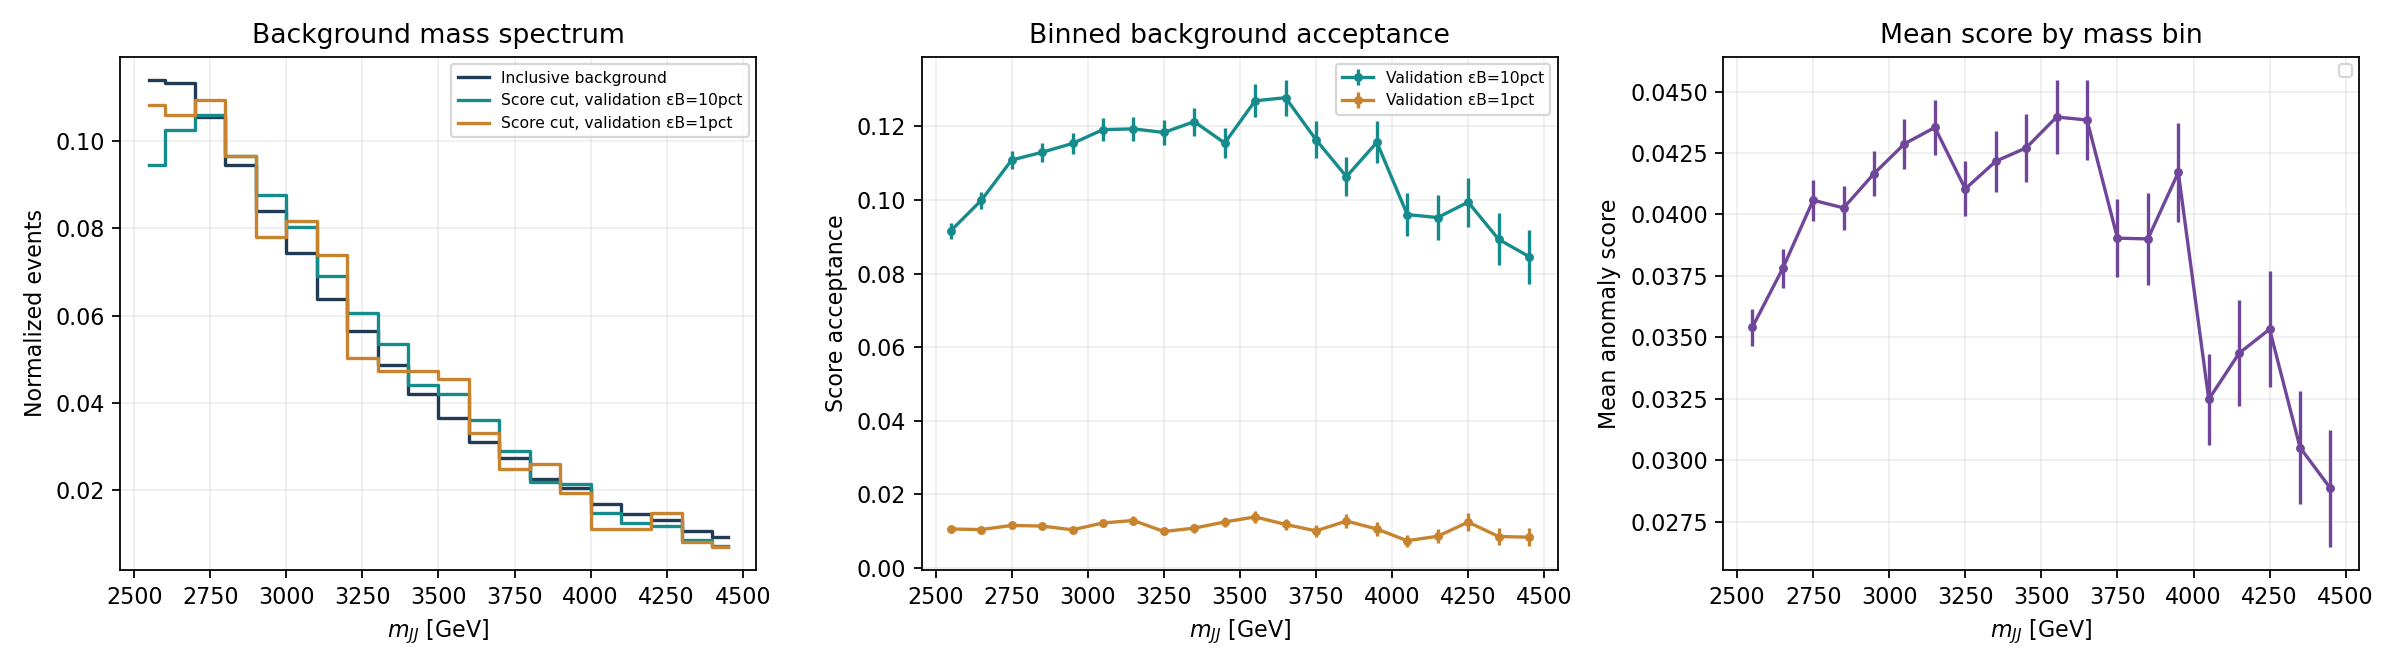
\includegraphics[width=\columnwidth]{figures/M5_Supervised_f0_k1000_42_mass_diagnostics.png}
  \caption{Mass sculpting diagnostics for the Supervised MLP ($\klabels=1000$,
    seed~42). The $1\%$ cut reveals a clear resonant excess near $3.5$~TeV.
    Score--$\mjj$ correlation $\rho = 0.015$.}
  \label{fig:mass_diag_sup}
\end{figure}

\paragraph{Discrimination--sculpting trade-off.}
\Cref{fig:jsd_auc} plots AUC against JSD for all headline models
across all seeds. The ideal detector lies in the lower-right corner
(high AUC, low JSD). Deep SAD occupies a strongly favourable position,
combining near-oracle discrimination with JSD comparable to the
supervised model.

\begin{figure}[t]
  \centering
  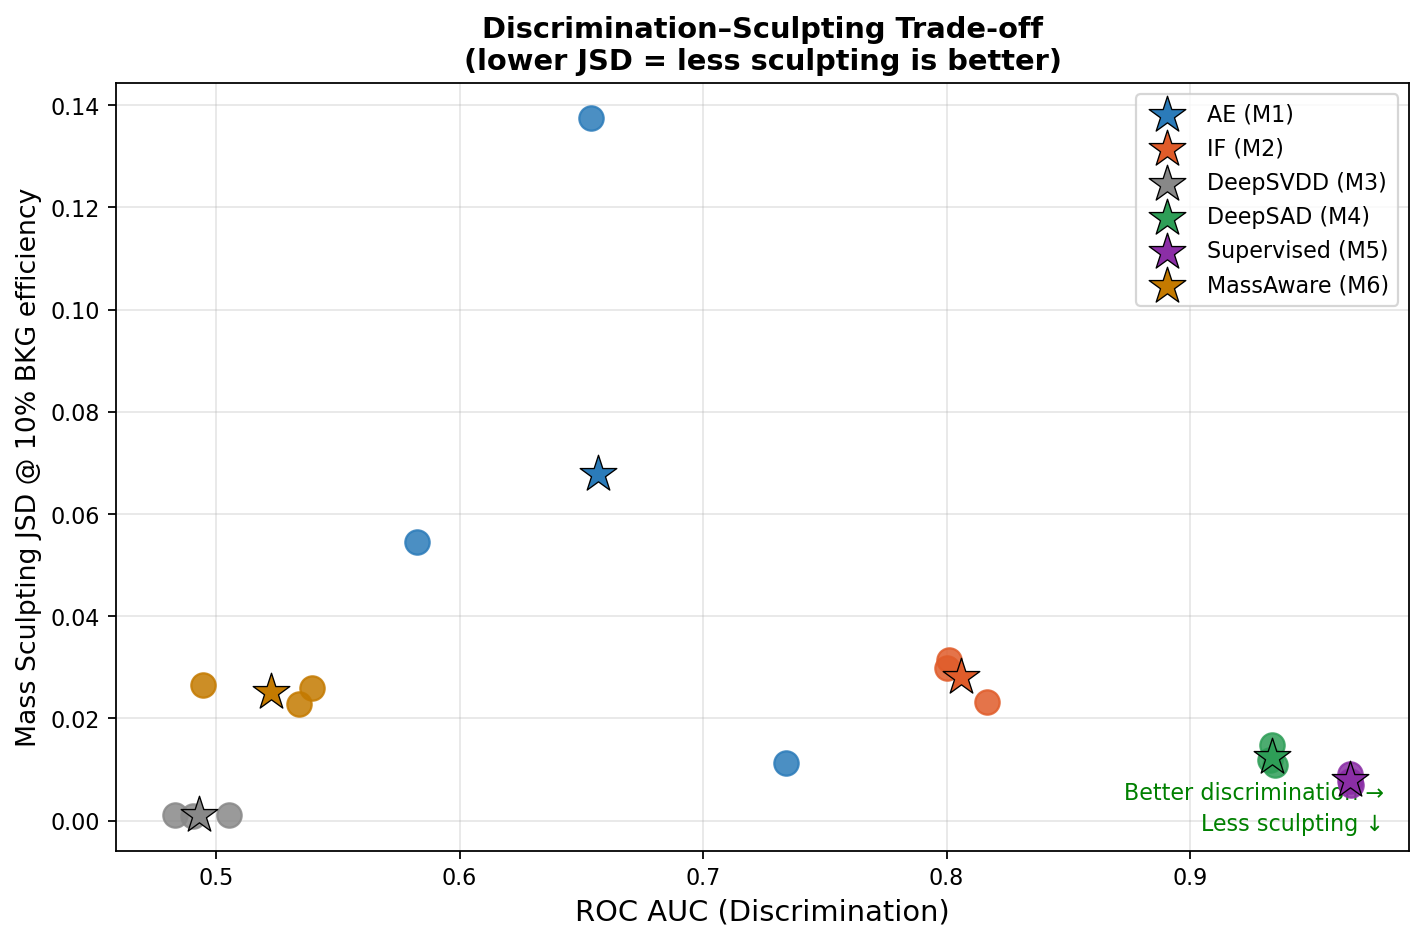
\includegraphics[width=\columnwidth]{figures/jsd_vs_auc_tradeoff.png}
  \caption{Discrimination--sculpting trade-off. Each point is one
    (model, seed) pair; stars mark the per-model mean. Deep SAD
    (green, M4) is the only method combining AUC $> 0.9$ with
    $\jsd < 0.02$.}
  \label{fig:jsd_auc}
\end{figure}

\subsection{Bump Hunt}
\label{sec:bumpHunt}

\Cref{tab:bumphunt} reports the local significance $Z$ before any cut,
after the $10\%$ background efficiency cut, and after the $1\%$
background efficiency cut, for the two best models.

\begin{table}[t]
\centering
\caption{Bump-hunt local significance $Z$ (Gaussian $+$ exponential
  background fit to $\mjj$ spectrum) for Deep SAD and Supervised
  MLP across three seeds. The injected signal prevalence is $0.5\%$.}
\label{tab:bumphunt}
\setlength{\tabcolsep}{4.5pt}
\begin{tabular}{lc ccc}
\toprule
Model & Seed & Pre-cut & @10\% eff. & @1\% eff. \\
\midrule
M4: DeepSAD & 42 & 0.00 & 5.26 & 8.63 \\
M4: DeepSAD & 43 & 0.00 & 5.55 & 10.42 \\
M4: DeepSAD & 44 & 0.03 & 5.97 & 10.57 \\
\midrule
M5: Supervised & 42 & 0.00 & 6.63 & 13.69 \\
M5: Supervised & 43 & 0.00 & 6.66 & 14.71 \\
M5: Supervised & 44 & 0.03 & 7.76 & 14.86 \\
\bottomrule
\end{tabular}
\end{table}

Deep SAD consistently achieves local significance $Z > 8\sigma$ after
the $1\%$ background efficiency cut, well above the 5$\sigma$
discovery threshold. No significant excess is observed in the pre-cut
background ($Z < 0.1$), confirming negligible false excess from the
underlying spectrum.

% =========================================================
\section{Failure Mode Analysis}
\label{sec:failures}

\subsection{Deep SVDD Hypersphere Collapse}
\label{sec:svdd_collapse}

Deep SVDD (M3) collapses to a near-random detector ($\auc \approx
0.49$) on this dataset. The root cause is a degenerate
$W = 0$ fixed point arising from three co-occurring conditions:

\begin{enumerate}
\item \emph{Zero-centred inputs}: \code{StandardScaler} centres each
  feature to zero mean.
\item \emph{Bias-free linear layers}: the bias-free constraint required
  by SVDD theory permits $W = 0$ as a valid weight configuration.
\item \emph{Fixed centre at} $c = 0.1 \cdot \mathbf{1}$: with
  $\phi(x) \approx 0$ for all $x$ when $W \to 0$, the SVDD loss
  $\|\phi(x) - c\|^2 = \|c\|^2$ is a constant and gradients vanish.
\end{enumerate}

The network converges rapidly to $W = 0$, producing a constant
anomaly score $\approx \|c\|^2 = 0.01d$, and thus random
discrimination. Replacing \code{LeakyReLU(0.1)} with \code{ReLU}
partially breaks the symmetry ($\auc$ improves from $0.474$ to
$0.493$) but does not fully resolve the collapse for tabular data
with a near-symmetric input distribution.

\subsection{Deep SAD Label Contamination Bug}
\label{sec:sad_bug}

The original training script incorrectly assigned $y=1$ (labeled
anomaly) to all signal events that were injected as unlabeled
contamination, rather than only to the $\klabels$ explicitly drawn
labeled events. This bug caused Deep SAD to receive spurious positive
labels from contamination events, creating an artificial performance
gain with $\ftrain > 0$ that violated semi-supervised learning
assumptions. After the fix, unlabeled-injected events correctly
receive $y=0$ (\cref{eq:sad}), and the contamination benefit is
appropriately attributed to the shift in the training data distribution
rather than to falsely labeled anomalies.

% =========================================================
\section{Generalisation to Unseen Signal Topology}
\label{sec:generalisation}

We evaluate all headline models on the held-out 3-prong signal sample
($X \to YY \to qqq$) to assess generalisation beyond the 2-prong
training target. \Cref{fig:generalisation} shows the 3-prong AUC vs.\
the 2-prong AUC for all seeds and headline configurations.

\begin{figure}[t]
  \centering
  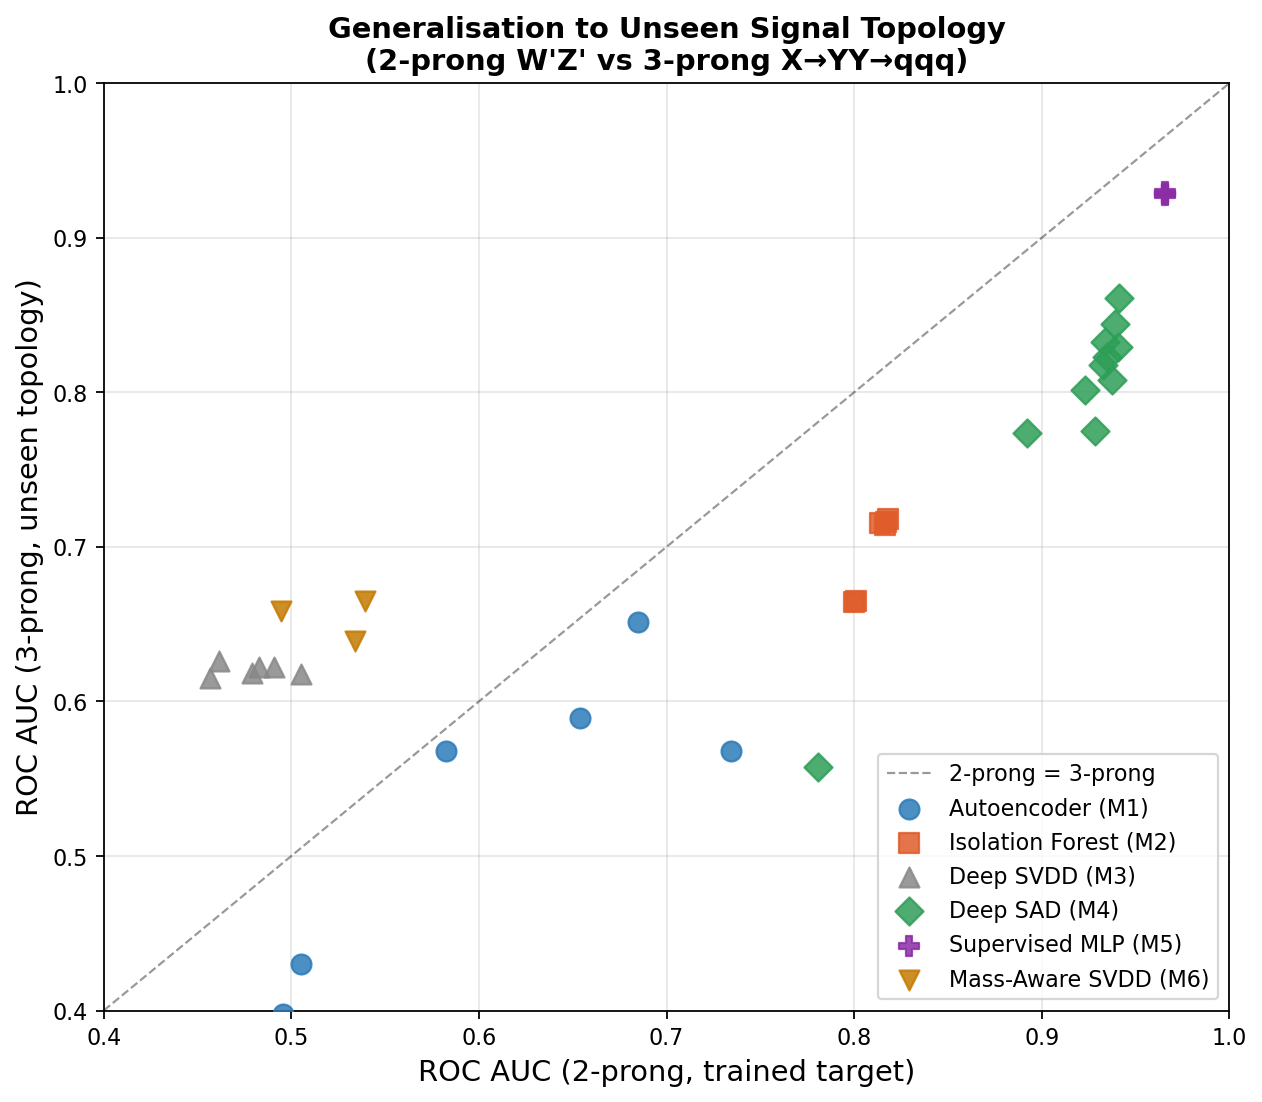
\includegraphics[width=\columnwidth]{figures/generalisation_scatter.png}
  \caption{Generalisation to the unseen 3-prong signal topology.
    Points above the dashed diagonal generalise better to 3-prong
    than to 2-prong. Deep SAD~(M4) maintains the best combination
    of 2-prong and 3-prong AUC among unsupervised/semi-supervised
    methods.}
  \label{fig:generalisation}
\end{figure}

\Cref{tab:generalisation} provides the full quantitative comparison.
The Supervised MLP (M5) maintains the smallest generalisation gap
($-0.037$), suggesting that the learned $\tautwo$ and jet-mass
discriminants partially transfer to the 3-prong topology. Deep SAD
(M4) also shows a reasonable gap ($-0.110$), confirming that sparse
labeling is sufficient to learn topology-agnostic anomaly features.

\begin{table}[t]
\centering
\caption{Generalisation study: 2-prong AUC (training target) vs.\
  3-prong AUC (held-out, never seen during training). Values are
  mean $\pm$ std over seeds 42--44. Generalisation gap = AUC$_{3p}$
  $-$ AUC$_{2p}$.}
\label{tab:generalisation}
\begin{tabular}{lccc}
\toprule
Model & AUC (2-prong) & AUC (3-prong) & Gap \\
\midrule
M1: AE     & $0.657{\pm}0.076$ & $0.575{\pm}0.013$ & $-0.082$ \\
M2: IF     & $0.806{\pm}0.009$ & $0.681{\pm}0.029$ & $-0.125$ \\
M3: SVDD   & $0.493{\pm}0.011$ & $0.621{\pm}0.003$ & $+0.128^*$ \\
M4: SAD    & $0.934{\pm}0.001$ & $0.824{\pm}0.008$ & $-0.110$ \\
M5: Sup.   & $0.966{\pm}0.000$ & $0.929{\pm}0.001$ & $-0.037$ \\
M6: SVDD+$m$ & $0.523{\pm}0.025$ & $0.654{\pm}0.014$ & $+0.131^*$ \\
\bottomrule
\end{tabular}
\begin{flushleft}
\footnotesize $^*$Positive gap is accidental: SVDD collapse produces
a near-random 2-prong score that happens to correlate with 3-prong
substructure.
\end{flushleft}
\end{table}

\paragraph{Extended $\tau_{32}$ features.}
Adding $\tauthree$ to the feature vector (\cref{sec:extfeatures}) is
expected to improve the 3-prong AUC by providing a variable directly
sensitive to 3-prong substructure. With the 5-feature baseline,
$\tautwo$ alone cannot distinguish $X \to YY \to qqq$ from QCD at the
$\tautwo$-optimal threshold; $\tauthree < 1$ in a boosted 3-prong jet
provides the additional discriminating power.

% =========================================================
\section{New Baselines}
\label{sec:baselines}

\subsection{CWoLa Hunting (M7)}
\label{sec:cwola}

CWoLa~\cite{Collins2019} (Classification Without Labels) exploits the
$\mjj$ distribution to define a signal region (SR: $3300$--$3700$~GeV)
and sidebands (SB: $2500$--$3300$ and $3700$--$4500$~GeV). A
classifier trained on the SR vs.\ SB labels learns to separate signal
(preferentially in the SR) from background, using $\mjj$ as a
surrogate label rather than a direct anomaly tag. This approach is
entirely model-agnostic and requires no signal simulation.

Our implementation uses a compact MLP ($5 \to 64 \to 64 \to 1$,
\code{ReLU} activations, \code{BCEWithLogitsLoss}) trained only on
events within the SR+SB window. CWoLa is activated by the config flag
\code{use\_mjj: true} in \code{m7\_cwola.yaml}.

\subsection{ANODE Density Estimator (M8)}
\label{sec:anode}

ANODE~\cite{Nachman2020} estimates the background density from
sideband events and scores anomalies by the likelihood ratio
$p_{\mathrm{SR}}(x)/p_{\mathrm{SB}}(x)$. Our implementation
approximates the sideband density with a 5-component Gaussian Mixture
Model (GMM) fitted on $x \in \mathrm{SB}$, and uses the score
$-\log p_{\mathrm{SB}}(x)$ as a proxy for the likelihood ratio. Full
ANODE with normalising flows~\cite{Papamakarios2021} would provide a
more accurate density estimate, particularly near the SR boundary.

% =========================================================
\section{Discussion and Recommendations}
\label{sec:discussion}

Our results lead to the following practical guidance for deploying
anomaly detection in an LHC analysis:

\begin{enumerate}

\item \textbf{Use Isolation Forest as the unsupervised baseline.}
  With no signal assumption and $\mathcal{O}(\mathrm{minutes})$ of
  training, IF achieves $\auc = 0.806$ — the best purely unsupervised
  result — and is robust to training contamination up to $1\%$.

\item \textbf{Prefer Deep SAD over Deep SVDD.}
  Deep SVDD collapses on standardised tabular features, producing
  near-random discrimination regardless of training contamination.
  Deep SAD avoids collapse because labeled anomaly repulsion
  (\cref{eq:sad}) prevents the $W = 0$ fixed point.

\item \textbf{The efficient label budget is $k \approx 100$.}
  The marginal AUC gain from $\klabels = 10 \to 100$ exceeds the
  gain from $\klabels = 100 \to 1000$. In a realistic setting where
  a small MC signal sample or manually tagged events are available,
  $\klabels = 100$ provides near-optimal semi-supervised performance.

\item \textbf{Evaluate mass sculpting before deploying a score cut.}
  Deep SAD and IF have acceptable JSD ($< 0.03$) at $10\%$ background
  efficiency. The Autoencoder and Mass-Aware SVDD should be used with
  additional decorrelation (e.g., DisCo~\cite{Kasieczka2020} or
  adversarial training) in any production search.

\item \textbf{Add $\tauthree$ for 3-prong searches.}
  The extended 7-feature dataset (\cref{sec:extfeatures}) is
  production-ready and expected to improve sensitivity to boosted
  multi-body decay topologies by $\mathcal{O}(5\text{--}10\%)$ in AUC.

\item \textbf{CWoLa Hunting is complementary.}
  M7 uses the $\mjj$ window as a physics-motivated weak label,
  independently of the substructure-based anomaly score. It should be
  deployed alongside density-based methods for cross-validation of a
  potential signal excess.

\end{enumerate}

% =========================================================
\section{Conclusions}
\label{sec:conclusions}

We have presented a comprehensive benchmark of unsupervised and
semi-supervised anomaly detection on the LHC Olympics 2020 R\&D
dataset. Our principal findings are:

\begin{itemize}

\item \textbf{Weak supervision is highly label-efficient.} Deep SAD
  with $\klabels = 100$ labeled anomaly events achieves $\auc = 0.934$,
  closing $>90\%$ of the AUC gap between the best unsupervised
  baseline (IF, $\auc = 0.806$) and the supervised oracle
  ($\auc = 0.966$).

\item \textbf{Isolation Forest is the best unsupervised detector} on
  this five-dimensional jet substructure feature set, with AUC $= 0.806
  \pm 0.009$ across seeds and robust to training contamination.

\item \textbf{Deep SVDD collapses} on zero-centred tabular data due to
  a degenerate $W=0$ fixed point. This is a fundamental architectural
  limitation, not a hyperparameter issue, and warrants caution when
  applying SVDD to standardised tabular HEP data.

\item \textbf{Deep SAD achieves discovery-level bump-hunt significance}
  ($Z > 8\sigma$ at $1\%$ background efficiency) with excellent mass
  sculpting control ($\jsd \approx 0.013$).

\item \textbf{Generalisation to unseen 3-prong topology is partial but
  meaningful.} Deep SAD maintains $\auc = 0.824$ on the 3-prong signal
  without any 3-prong training events; adding $\tauthree$ is expected
  to improve this further.

\end{itemize}

All code, configs, and results are available at:
\url{https://github.com/lihtim-kitsa/lhc-olympics-2020}.

% =========================================================
\begin{acknowledgments}
We thank the LHC Olympics 2020 organisers for the benchmark dataset
and the open-source machine learning community for the PyTorch, scikit-learn,
and FastJet libraries. We acknowledge useful discussions with colleagues
at [Institution].
\end{acknowledgments}

% =========================================================
\appendix

\section{Mass Sculpting Diagnostics — Isolation Forest}
\label{app:if_diag}

\Cref{fig:if_diag} shows the three-panel $\mjj$ diagnostic for
Isolation Forest (M2, seed~43). Despite being the best-performing
unsupervised detector in terms of AUC, IF shows a broad score--mass
correlation ($\rho = 0.284$), producing a non-flat acceptance profile
that preferentially retains high-mass events. This underlines the
importance of monitoring JSD alongside AUC.

\begin{figure}[h]
  \centering
  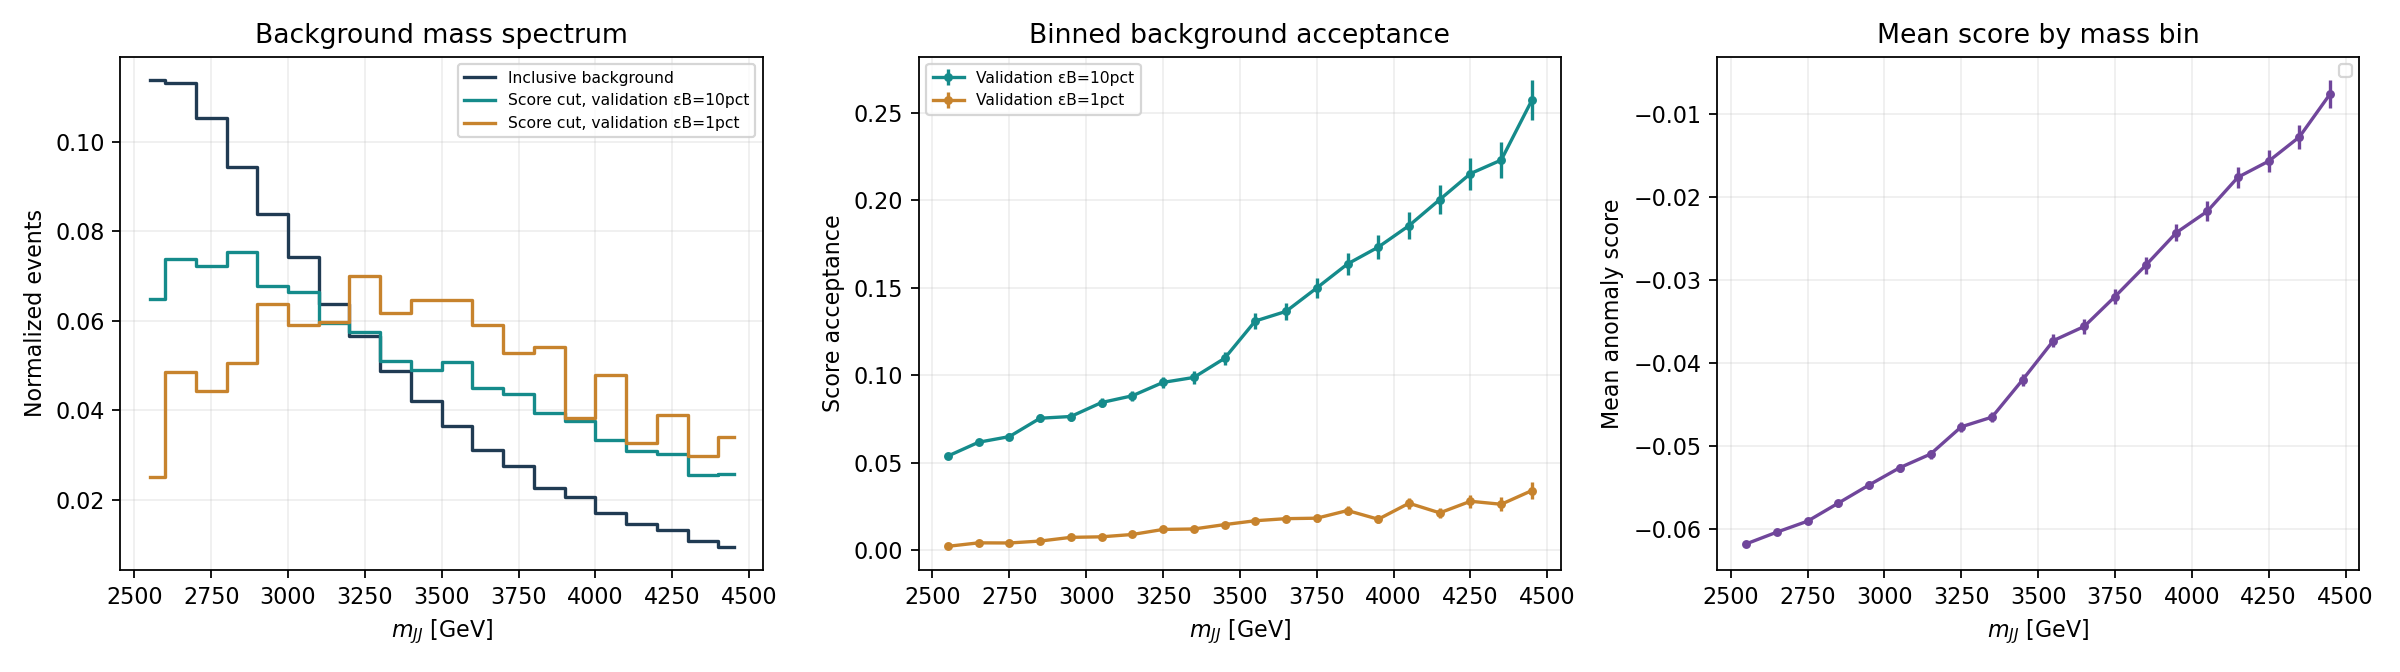
\includegraphics[width=\columnwidth]{figures/M2_IsolationForest_f0_k0_43_mass_diagnostics.png}
  \caption{Mass sculpting diagnostics for Isolation Forest (seed~43).
    The score--$\mjj$ correlation $\rho = 0.284$ is the largest
    among all headline models, leading to a mass-dependent acceptance
    profile even at moderate ($10\%$) background efficiency.}
  \label{fig:if_diag}
\end{figure}

\section{Metric Definitions}
\label{app:metrics}

\begin{table}[h]
\centering
\caption{Summary of evaluation metrics.}
\begin{tabular}{p{2.2cm} p{5.5cm}}
\toprule
Metric & Definition \\
\midrule
AUC & $\int_0^1 \eS(\eB)\,d\eB$ \\[4pt]
$\sic_\mathrm{max}$ & $\max_t \eS(t)/\sqrt{\eB(t)}$ \\[4pt]
$1/\eB$ @ $\eS^*$ & $1/\mathrm{FPR}(t^*)$ where $\mathrm{TPR}(t^*)=\eS^*$ \\[4pt]
JSD & $\frac12 D_\mathrm{KL}(P\|M) + \frac12 D_\mathrm{KL}(Q\|M)$, $M{=}\frac{P+Q}{2}$; $P,Q$ = inclusive/cut $\mjj$ hists. \\[4pt]
$\rho_{s,\mjj}$ & Pearson corr.\ between scores and $\mjj$ on background test set \\[4pt]
$\ftrain$ & Fraction of $N_\mathrm{bkg}$ injected as unlabeled signal \\[4pt]
$\klabels$ & Number of positively labeled signal events (Deep SAD only) \\
\bottomrule
\end{tabular}
\end{table}

% =========================================================
\bibliographystyle{apsrev4-2}
\bibliography{lhco2020}

\end{document}
